% This is samplepaper.tex, a sample chapter demonstrating the
% LLNCS macro package for Springer Computer Science proceedings;
% Version 2.20 of 2017/10/04
%
\documentclass[runningheads]{llncs}
% Add your own packages here
\usepackage{graphicx}
%
\begin{document}
%
\title{Process Discovery using Big Data stack - Implementing the Alpha Algorithm with Map-Reduce}
\subtitle{Project Initiation}
%
%\titlerunning{Abbreviated paper title}
% If the paper title is too long for the running head, you can set
% an abbreviated paper title here
%

\author{Martin Hashem, Xiangan Chen}

\institute{
\today \\
RWTH Aachen \\
%\date{01 Apr 2019}
}
%
\maketitle              % typeset the header of the contribution
%
%\begin{abstract}
%The abstract should briefly summarize the contents of the paper in
%150--250 words.
%\end{abstract}
%
%	
%
\section{Overview}
Process mining is an approach to extract process models from event logs. Since the distributed nature of modern information systems, event logs are likely to be distributed among different physical machines. Map-Reduce is a scalable approach for efficient computations on distributed data. In this Python application we will present the main idea of a Map-Reduce implementation of the Alpha process mining algorithm, to take advantage of the scalability of the Map-Reduce approach.\\

\noindent
To fulfill the shortcoming in the current process mining technology, this project aims to build a new python-based web service, that integrates the big data capabilities of the Hadoop system into the process mining framework pm4py.
\section{Buisness Case}
We develop a business case to disclose the potential of this project. The study is divided into three parts. First we explain one of the current algorithm in process mining. Furthermore we will define the scope of the project and point out the key benefits of our optimization.
\subsection{Initial Situation}
The current situation in process mining eventlogs using the Alpha algorithm is very centralized. All eventlogs are pushed together into one computation unit, eating up a big amout of resources, both in used space and computation time. The optimization of this is the main task.
\subsection{Scope}
The main goal of this project is to create a web application that provides calculations with the Alpha algorithm and can prepare the data using the Map-Reduce. The project contains these tasks:\\
\begin{itemize}
	\item[\Large $\cdot$] \textbf{Code required:} Intergrating the system Hadoop into the pm4py interface and read files from it
	\item[\Large $\cdot$] \textbf{Code required:} Run the Alpha algorithm utilizing Map-Reduce 
	\item[\Large $\cdot$] \textbf{Code required:} Reading in logs and upload them into Hadoop
\end{itemize}
The web service is to be accessed by a standard browser and needs to provide the folowing functionalities:
\begin{itemize}
	\item[\Large $\cdot$] Upload event logs in either CSV or XES format into the Hadoop system
	\item[\Large $\cdot$] Front end links to existing algorithms for further processing
	\item[\Large $\cdot$] Do Map-Reduce computations to run the alpha algorithm
	\item[\Large $\cdot$] Download the files onto local system
\end{itemize}
Additionally these documentations will be provided to bring insights to our software development cycle:
\begin{itemize}
	\item[\Large $\cdot$]  Project initiation document
	\item[\Large $\cdot$]  Requirements analysis document
	\item[\Large $\cdot$]  Design document
	\item[\Large $\cdot$]  Software documentation
\end{itemize}
\subsection{Key Benefits}
The current scope of mining in Big Data is slow and centralized. Using map-reduce in combination with the Alpha algorithm, calculations can be deffered to more, smaller instances and also reduce overhead in transferring the events. Depending on the amount of  map-reduce stages that are implemented, there can be significantly less time used during the mining process, due to the parallized nature of the approach. \cite{mapReduce}
\section{Feasibility Study}

\subsection{Theoretical Point of View}
A paper by Assadipour\cite{mapReduce} suggests that using a decentralized approach for process mining using the Alpha algorithm by splitting the calculations into smaller tasks available to smaller instances. \\ \ \\
The Alpha algorithm takes eventlogs and generates a Petri net model including an initial and final mark. The main purpose of the Alpha algorithm is to portray the relations between activities, but comes with the flaw of not finding self loops.  \\ \ \\
Map-Reduce is a technique to allow the user to have a scalable calculation on a distributed system. By first mapping events to an identifier and then reducing the map to its relevant values, the amount of needed data shrinks. Here the reductions prepare the data for the Alpha algorithm, removing the overhead of finding the traces first.
\subsection{Technical Point of View}
For our project we mostly rely on well-established open source technology. This includes primarily the following tools:\\

\begin{itemize}
	\item[\Large $\cdot$]   Python 3.6 as back end programming language
	\item[\Large $\cdot$]   pm4py python library as process mining toolkit
	\item[\Large $\cdot$]   Flask as web framework
	\item[\Large $\cdot$]   Hadoop as big data processing and distributed computation framework
	\item[\Large $\cdot$]   Docker as virtual machine and deploy platform\\
\end{itemize}

\noindent
The pm4py library is a joint effort of the Fraunhofer FIT process mining group\cite{FIT} and the RWTH Process and Data Science group\cite{pads}, which supports state-of-the-art process mining algorithms in python. It is completely open source and intended to be used in both academic and industrial projects.\\

\noindent
Flask\cite{Flask} is a micro web framework written in Python. It is classified as a microframework because it does not require particular tools or libraries. It has no database abstraction layer, form validation, or any other components where pre-existing third-party libraries provide common functions. It is very suitable for our web application.\\

\noindent
Apache Hadoop\cite{Hadoop} is a collection of open-source software utilities that facilitate using a network of many computers to solve problems involving massive amounts of data and computation. It provides a software framework for distributed storage and processing of big data using the Map-Reduce programming model. So we take its advantages in our project so that we can deal with the big data and distributed event log properly.\\

\noindent
Docker\cite{Docker} is a computer program that performs operating-system-level virtualization. Docker is used to run software packages called containers. Containers are isolated from each other and bundle their own application, tools, libraries and configuration files; they can communicate with each other through well-defined channels. We will deploy our application on a production-grade server with Docker.

\subsection{Risks and Mitigations}
For our risk analysis we distinguish between project management related risks and technical risks. In order to reduce potential issues we define a list of strategies and countermeasures as general risk management.

\subsubsection{Project Managment Risks}

The following table covers potential organizational risks and countermeasures:\\

\renewcommand\arraystretch{1.5}
\begin{tabular}{p{5cm}|p{6cm}}
	Risk& Mitigation\\
	\hline
	Project team may misunderstand requirements.& Requirement misinterpretation can be mitigated by discussing between group members and frequent meetings with our advisors. Open questions should be addressed as soon as possible.\\
	\hline
	Learning curves lead to delays and cost overrun.& The degree of modularization depicted according to the project plan allows each team member to focus on a half set of skills only.\\
	\hline
	Time conflicts between team members.& Regular feedback communications.\\
	\hline
	Features are developed twice or not at all.& Since we have a two-man team, we will devide the tasks clearly and discuss them often.\\
\end{tabular}

\subsubsection{Technical Risks}

Since the Apache Hadoop and Flask are open source softwares, they bring us some significant advantages such as free to use, but they also have some limitations as compared to the commercial ones. In the following table technical related risks are considered:\\

\renewcommand\arraystretch{1.5}
\begin{tabular}{p{5cm}|p{6cm}}
	Risk& Mitigation\\
	\hline
	No formal support contracts.& Restrict to well-documented and established open
	source software.\\
	\hline
	Graphical user interface is not user-friendly.& Improve user interface in the frontend in an agile manner.\\
	\hline
	Software components do not work together.& Define clear and well structured interfaces in the early design phase.\\
	\hline
	Uploaded file not recognizable.& Appoint a obvious sign on the frontend site to notify the user to upload the correct format.\\
\end{tabular}

\section{Project Plan}
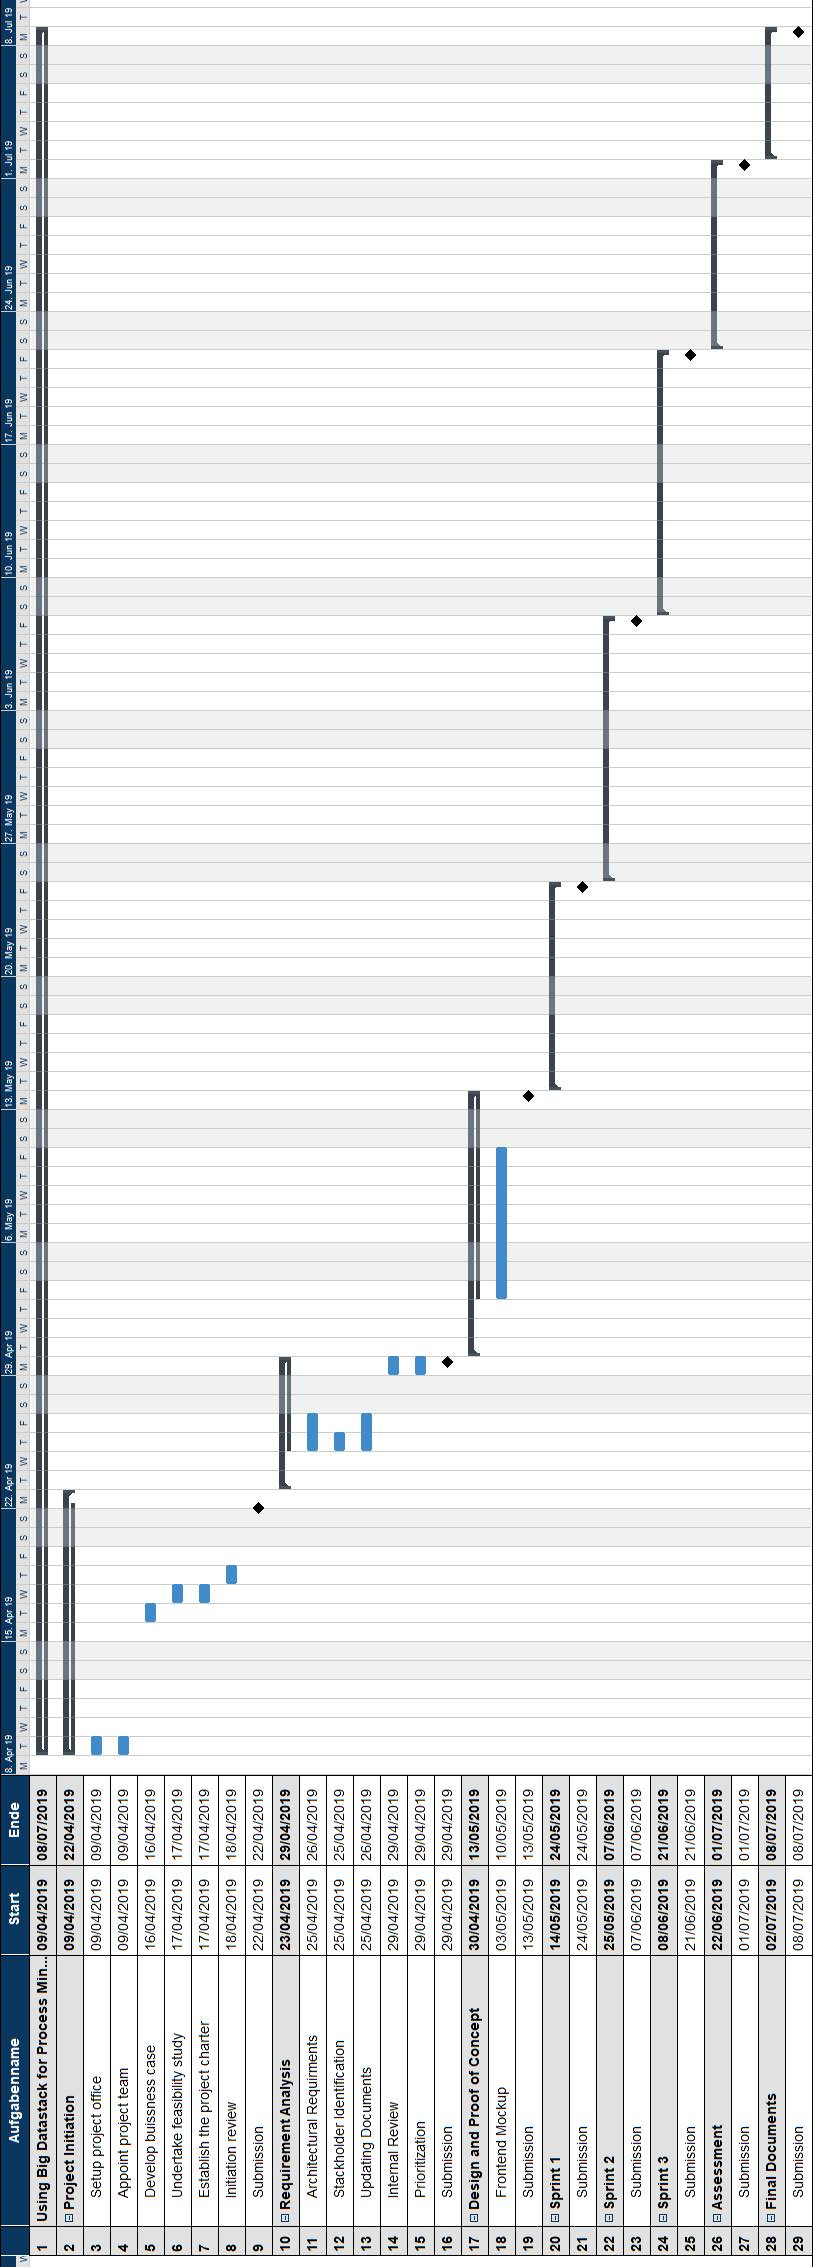
\includegraphics[scale=.3333]{Gantt.jpg}
\section{Project Team}
The project team consists of two persons. The following roles have been assigned to reflect individual strengths and competences:\\


\renewcommand\arraystretch{2}
\begin{tabular}{c|cc}
	Name& Role& Contact\\
	\hline
	Martin Hashem& Project Manager& martin.hashem@rwth-aachen.de\\
	& Backend Architect& \\ 
	Xiangan Chen& Quality Manager& xiangan.chen@rwth-aachen.de\\
	& Frontend Architect & \\
\end{tabular}
\\\\[2pt]
In addition a team member is assigned to each milestone in the project, who is primarily
responsible, that the requirements and goals of the milestone are met in time with sufficient quality. The responsibilities are stated in the following table:\\

\begin{tabular}{lc}
	Milestone& Chief Responsibility\\
	\hline
	Project initiation document& Xiangan Chen\\
	Requirement analysis document& Xiangan Chen\\
	Design and proof of concept& Martin Hashem\\
	Sprint 1& Martin Hashem\\
	Sprint 2& Xiangan Chen\\
	Sprint 3& Martin Hashem\\
	Assessment& Xiangan Chen\\
	Final Documents& Martin Hashem\\
\end{tabular}


% Start bibliography
\bibliographystyle{alpha}
\bibliography{ProjectInitiation}

\end{document}
